\documentclass{entcs} 
\usepackage{entcsmacro}
\usepackage{graphicx}
\usepackage{algorithm}
\usepackage{algorithmic}

% The following is enclosed to allow easy detection of differences in
% ascii coding.
% Upper-case    A B C D E F G H I J K L M N O P Q R S T U V W X Y Z
% Lower-case    a b c d e f g h i j k l m n o p q r s t u v w x y z
% Digits        0 1 2 3 4 5 6 7 8 9
% Exclamation   !           Double quote "          Hash (number) #
% Dollar        $           Percent      %          Ampersand     &
% Acute accent  '           Left paren   (          Right paren   )
% Asterisk      *           Plus         +          Comma         ,
% Minus         -           Point        .          Solidus       /
% Colon         :           Semicolon    ;          Less than     <
% Equals        =3D           Greater than >          Question mark ?
% At            @           Left bracket [          Backslash     \
% Right bracket ]           Circumflex   ^          Underscore    _
% Grave accent  `           Left brace   {          Vertical bar  |
% Right brace   }           Tilde        ~

% My own definitions
\newcommand {\keyw}[1]{{\bf #1}}

% A couple of exemplary definitions:

\newcommand{\Nat}{{\mathbb N}}
\newcommand{\Real}{{\mathbb R}}

\def\lastname{Palshikar and Bhaduri}
\begin{document}
\begin{frontmatter}
  \title{Verification of Scenario-based Specifications using Templates} 
  \author{Girish Keshav Palshikar \thanksref{myemail}}
  \author{Purandar Bhaduri \thanksref{coemail}}
  \address{Tata Research Development and Design Centre (TRDDC),\\ 
  54B, Hadapsar Industrial Estate, Pune 411013, India.}
  \thanks[myemail]{Email:
  \href{mailto:girishp@pune.tcs.co.in} {\texttt{\normalshape
        girishp@pune.tcs.co.in}}}
  \thanks[coemail]{Email:
    \href{mailto:pbhaduri@pune.tcs.co.in} {\texttt{\normalshape
        pbhaduri@pune.tcs.co.in}}}

\begin{abstract} 
Specifying dynamic behaviour of a system by listing scenarios of 
its interactions has become a popular practice. Message sequence 
chart (MSC) is a rigorous and widely used notation for specifying 
such scenarios of system behaviour. High-level MSCs (HMSC) 
provide hierarchical and modular composition facilities for 
constructing complex scenarios from basic MSCs. Although the 
general problem of formal verification of properties of HMSCs is 
intractable, we propose a framework for restricted verification. 
We present simple templates for commonly used types of properties 
and discuss efficient algorithms for verifying them.
\end{abstract}
\begin{keyword}
Scenario-based Specifications, Message Sequence Charts, 
Formal Verification, Formal Methods.
\end{keyword}
\end{frontmatter}

\section{Introduction}\label{intro}

It is important to clearly and precisely state the behavioural 
requirements when building practical business systems as well as 
safety-critical real-time, embedded systems (e.g., see our 
railway system~\cite{Girish03}). It is not always easy to communicate 
dynamic behavioural requirements of a system to the end-users 
in an easy-to-understand non-mathematical manner, particularly 
in the early stages of requirements analysis, where the 
requirements need to be high-level and abstract (removed from 
design and implementation issues). A simple and intuitive way 
to describe a system is to list various examples or scenarios 
of its intended behaviour. At the highest level of abstraction, 
a scenario describes a set of interactions of the system with 
its environment and other external systems. An interaction 
includes entities (including system components) that 
participate in it and event occurrences. An interaction 
scenario often stands for a set of possible event sequences 
(episodes). Each interaction scenario is typically classified 
as either desirable ({\em sunny day}) or undesirable ({\em rainy day}). 
Ideally, an implementation should meet all sunny day interaction 
scenarios and none of the rainy day ones.

There is a need for simple, expressive, intuitive, graphical 
and standardised notations to specify interaction scenarios 
of systems. Message sequence chart (MSC) is just such a simple, 
visual and mathematically rigorous
notation~\cite{Rudolph96a,Haugen:2001:MID}. MSCs have 
been used widely in the telecom domain and are also 
increasingly being used in many other applications~\cite{Girish03}. The 
sequence diagram and use case notations in UML are semantically 
and visually close to the MSC
notation~\cite{Haugen:SDL:2001,Graubmann:2000:UML,Miga:2001:DMS,Feijs00}. 
The ITU standard for MSC~\cite{MSC96} includes a mathematical semantics for it. 
Other researchers have provided mathematical semantics for 
MSCs using formalisms such as transition systems, process 
algebras
etc.~\cite{Jonsson:2001:ESM,Mauw:1999:OSM,Mauw96,gehrke98algebraic}.  
In this paper, we use the 
partial order semantics given by Alur et al~\cite{Alur96}. The main 
use of a formal semantics for a notation is that it can be 
used to design formal verification and analysis algorithms. 
For example, a specification written using MSCs can be 
analysed to detect various problems such as missing scenarios 
and race conditions. Formal verification algorithms can be 
designed which check whether a given specification written 
using MSCs satisfies a given property written in a suitable formal
notation~\cite{Alur96,AEY01b,Peled00,LevPel97,1997:tacas:ben-abdallah,MuschollPeled00,MSP98,BVP02}.
Model-checking tools have also been applied for formal verification of
MSCs~\cite{AlurYannakakis99,GenestEtAl02}.

This paper presents a set of restricted simple property 
templates and formal verification algorithms to check whether a 
given High-level MSC (HMSC) satisfies the given property. 
Since the general problem of formal verification of HMSC 
specification is intractable when the property is specified 
in temporal logic or equivalent notations,
following~\cite{patterns-spec,model-checking-managers,BVP02},
we restrict the kinds of properties that can be 
specified and give specialised algorithms for formal 
verification of properties specified using each template. We 
present a compromise wherein we sacrifice expressiveness 
for efficient verification. The MSC notation has been 
extended in several ways (e.g.,~\cite{Silva98}); here we focus on the 
core aspects of the MSC and HMSC notation only. 

Section~\ref{hmsc-sem} presents an overview of HMSC notation and its 
formal semantics. Section~\ref{hmscveri} discusses our approach of 
property templates and algorithms to verify them.
Section~\ref{con} provides conclusions and further work.

\section{HMSC Semantics}\label{hmsc-sem}

We assume familiarity with basic MSC notation and its 
partial order (linear time) semantics~\cite{Alur96}
(see Appendix~\ref{app} for an overview).
Here we summarise the relevant definitions
for MSC-graphs and HMSC.

\subsection{Linear Time Semantics of MSC Graphs}\label{mscgraph1}

An MSC graph is essentially a directed (not necessarily 
acyclic) graph in which each vertex refers to a basic MSC. 


\begin{definition}
\label{mscgraph}
An {\em{MSC graph}} $G$ is a tuple $(V,\rightarrow,v^I,v^T,\mu)$ 
where $V$ is a finite set of vertices, $\rightarrow$ is a 
binary relation over $V$ (each element of $\rightarrow$ is 
a directed edge in $G$), $v^I$ is the initial vertex, 
$v^T$ is the terminal vertex and $\mu$ is a labelling 
function that maps each vertex to a basic MSC $m$.
\end{definition}

When defining the semantics of MSC graphs, there are two ways of interpreting the
concatenation of basic MSCs $m_1$ and $m_2$. In \emph{synchronous} concatenation,
all the events in $m_1$ precede any event in $m_2$. The \emph{asynchronous} concatenation
corresponds to concatenating two MSCs instance by instance.

\begin{definition}
\label{msc-synch-concat}
The partial order associated with the \emph{synchronous
concatenation} of two basic MSCs $m_1$ and $m_2$ having
the same set of instances is the partial order
$\leq_{m_1,m_2}$ on $locations(m_1) \uplus locations(m_2)$ given by 
$$ \leq_{m_1} \uplus \leq_{m_2} \uplus~ locations(m_1) \times locations(m_2)$$
where $locations(m)$ is the set of locations (events)
in basic MSC $m$ and $\uplus$ is the operator for disjoint
union of two sets. Each location is denoted by a tuple 
$<i,l>$ where $i$ is the unique ID for an instance and
$l$ is the ID for the event within the visual order of
the instance $i$ (see Appendix~\ref{app}).
\end{definition}

\begin{definition}
\label{msc-asynch-concat}
The partial order associated with the \emph{asynchronous 
concatenation} of two basic MSCs $m_1$ and $m_2$ having 
the same set of instances is the partial order 
$\leq_{m_1,m_2}$ on $locations(m_1) \uplus locations(m_2)$ 
given by the transitive closure of the following relation:\\
$\leq_{m_1} \uplus~ \leq_{m_2} \cup~ \{(<i,l>_{m_1},
<i,l>_{m_2}) ~|~ <i,l>_{m_1} ~\in~ locations(m_1) \\
~\wedge \mbox{$<i,l>_{m_2}$} ~\in~ locations(m_2)\}$ 
\end{definition}

Figure~\ref{fig1} shows an MSC graph (initial vertex and terminal 
vertex are not shown, initial vertex connects to $v0$ and 
vertices $v2$, $v3$ connect to the terminal vertex). There 
are an infinite number of paths from the initial to the 
terminal vertex in this MSC graph (due to the loop in it); 
e.g., $<v0,v1,v3>$, $<v0,v1,v0,v1,v3>$, 
$<v0,v1,v0,v1,v0,v1,v3>$ etc. The idea in the semantics 
of MSC graph with synchronous concatenation is to construct a partial order for each 
such finite path in the MSC graph, by synchronously 
concatenating the partial orders of the basic MSCs 
occurring in the path. Figure~\ref{fig1} also shows the precedence 
graph for walk $<v0,v1,v0,v1,v3>$ in the MSC graph; this 
graph is obtained by synchronously concatenating the 
basic MSCs for $v0$, $v1$, $v0$, $v1$ and $v3$. Dashed 
lines show the edges in the precedence graph added due 
to Definition~\ref{msc-synch-concat}; we omit the edges entailed
by transitive closure. Note that the locations (events) 
are renamed in different instance of $v0$ (and $v1$) in 
the walk (due to the disjoint union).

\begin{figure*}[t]
\centering
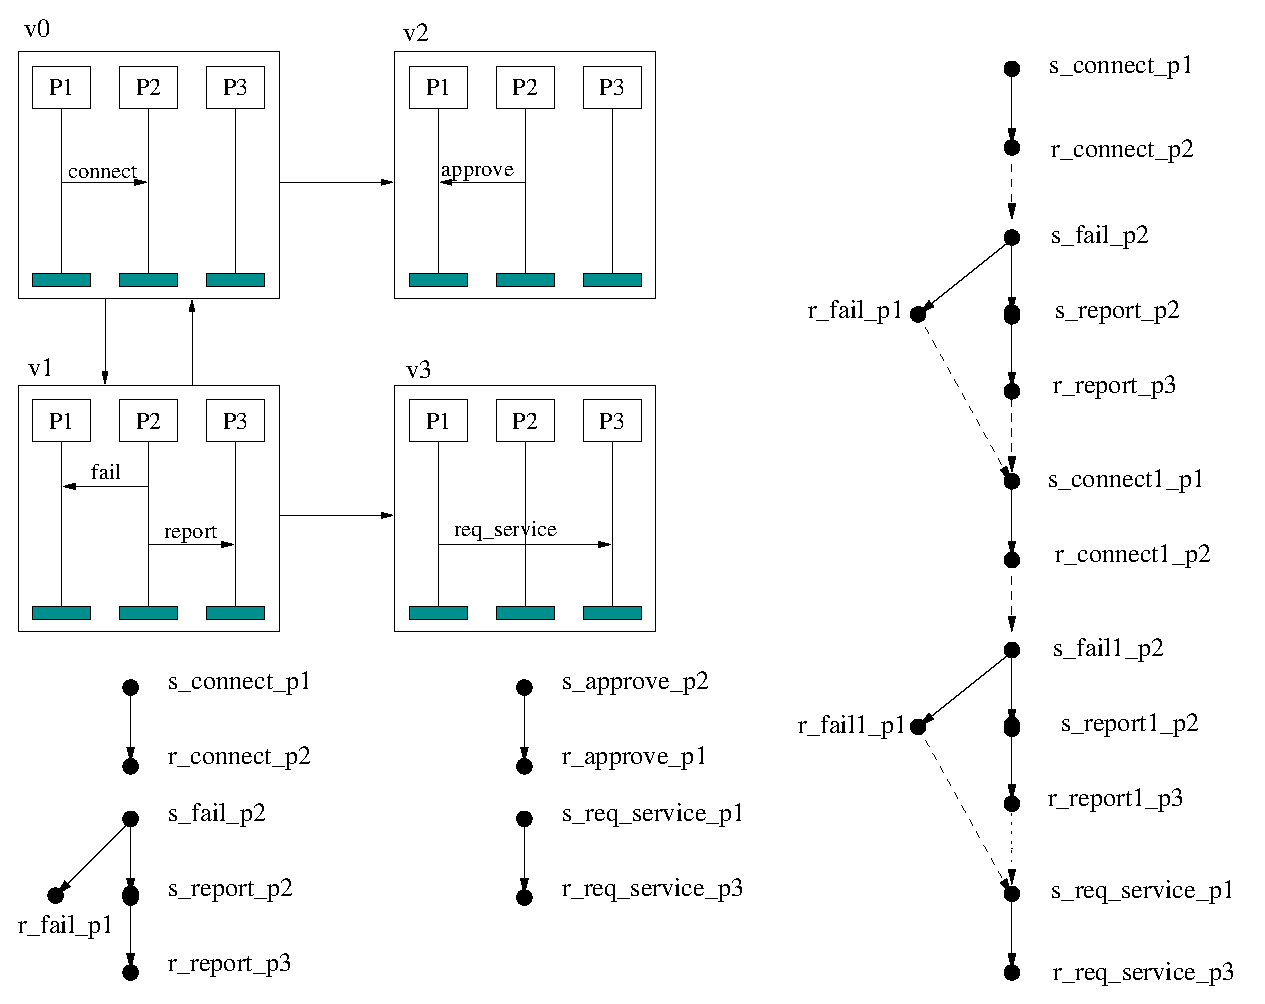
\includegraphics[height=10cm]{fig1}
\caption{MSC Graph}
\label{fig1}
\end{figure*}

\begin{definition}
\label{mscgsemantics}
The semantics of an MSC graph $G$ under (a)synchronous concatenation is the set of all 
finite and infinite runs obtained by (i) (a)synchronously 
concatenating each basic MSC along each walk in $G$ and 
(ii) taking the disjoint union over all walks, both 
finite and infinite, of the set of runs obtained from 
the partial orders in (i).
\end{definition}

Since the set of walks in an MSC graph may be infinite 
(if it has loops), the set of runs is also infinite. 
The problem of deciding whether a given MSC-graph 
satisfies a given property $P$ (where $P$ is specified 
as an automaton) is coNP-complete for synchronous concatenation 
and is undecidable for asynchronous concatenation~\cite{AlurYannakakis99}.

\subsection{Linear Time Semantics of HMSC}\label{hmsc1}

Essentially, an HMSC is a hierarchical (multi-level) 
graph whose nodes are either basic MSCs or another HMSC, 
thus allowing for nesting of graphs. 

\begin{definition}
\label{hmsc-def}
A {\em {high-level message sequence chart (HMSC)}} $H$ is a 
tuple $(N,B,v^I,v^T,\mu,E)$ where $N$ is a finite 
set of nodes, $B$ is a finite set of boxes 
(or supernodes), $v^I \in N \cap B$ is the initial 
node or box, $v^T \in N \cap B$ is the terminal 
node or box, $\mu$ is a labelling function that maps 
each node in $N$ to a basic MSC and each box in $B$ 
to an already defined HMSC, and $E$ is the set of 
edges that connect the nodes and boxes to each other.
\end{definition}

We omit some HMSC features in the MSC standard such as 
conditions and inline expressions. What is the meaning 
of an HMSC $H$? First, an HMSC is {\em flattened} into an 
MSC-graph, obtained by recursively substituting a box 
by the corresponding HMSC. The meaning of an HMSC is 
then the set of all possible finite or infinite runs 
of this flattened MSC-graph~\cite{AlurYannakakis99};
here it is required that the 
nesting of HMSCs is not mutually recursive, i.e., 
if a node of an HMSC $H$ is labelled with another HMSC 
$H$', then a node of $H$' cannot be labelled with $H$ 
(or with any HMSC that refers to $H$).

\section{HMSC Verification}\label{hmscveri}

Given an HMSC $H$ and a property $P$ about the runs of 
$H$, the verification problem is to decide whether or 
not all runs of $H$ satisfy $P$. $P$ is typically 
stated using temporal logic like LTL or CTL, an 
automaton or a template MSC. A na{\"\i}ve verification 
algorithm would examine some or all runs of $H$ to 
decide whether or not $H$ satisfies $P$. The general 
problem of deciding whether a given MSC-graph satisfies 
a given property $P$ (where $P$ is specified as an 
automaton) is undecidable\cite{AlurYannakakis99}. However, we consider 
some special classes of properties below and present 
efficient verification algorithms for such properties. 
Following~\cite{patterns-spec,model-checking-managers,BVP02}, we assume that the properties fall 
into various pre-defined templates, thus sacrificing 
generality for ease of use and efficiency of verification. 
The properties are stated in terms of the relative 
ordering of events in the runs of the input HMSC. 
Although the property templates cannot express all the 
properties that may be of interest in practice, they 
do cover broad classes of typical properties. Moreover, 
we present efficient graph-theoretic algorithms (based 
on linear time semantics of HMSCs) to verify properties 
stated using these templates. 

Every internal event in an HMSC has a unique ID 
specified by the unique location in the basic MSC in 
which it occurs. A user-defined event $E$ corresponds 
in general to a non-empty finite set $\gamma(E)$ of 
internal events in an HMSC. The properties are specified 
in terms of user-defined events and their negations. 
We say that a user-defined event occurs when any of 
the internal events corresponding to it occur. If a 
user-defined event $E$ stands for a finite set 
$\{e_1,\ldots,e_k\}$ of internal events, the negative event 
$not(E)$ stands for $not(e_1) \wedge \ldots \wedge not(e_k)$. 
In Figure~\ref{fig1}, a user event ``$P2$ sends message $\_$ to $P1$'' 
(underscore $\_$ stands for ``don't care'') corresponds 
to the two internal events: ``$P2$ sends $approve$ to $P1$'' 
(in basic MSC $v2$) and ``$P2$ sends $fail$ to $P1$'' 
(in basic MSC $v1$).

\paragraph{Note} In this paper, all our verification algorithms assume
\emph{synchronous} concatenation in the semantics of MSC graphs. This makes the algorithms
modular in nature, in the sense that the verification task can be decomposed into
smaller tasks that can be verified at each vertex. The verification algorithms for
asynchronous concatenation are more complex, as they involve the construction of a global
reachability graph from the input MSC graph.

\subsection{Tracing}\label{tracing}

A tracing property asserts the occurrence of a sequence 
of events in the specified order in all runs or in at 
least one run of the input HMSC $H$. The template for 
the property is shown below. The terms in bold are given 
by the user and the terms in bold separated by slashes 
are alternatives, one of which is chosen by the user. 
Each $a_i$ is a user-defined event or its negation.

%NOTE: insert table here
\begin{tabular}{|l|}
\hline
The sub-sequence of events {\bf $X = {\bf [a_1,a_2,\ldots,a_k]}$} 
occurs in {\bf some} / {\bf all} \\
runs of HMSC {\bf $H$} \\
\hline
\end{tabular}

\begin{definition}
\label{userevent}
Let $H$ be an MSC-graph and let 
$\sigma = u_0,u_1,u_2,\ldots$ be a run of $H$, where each $u_i$ 
is an internal event in some MSC $M$ in $H$. A positive 
user-defined event $a = \{e_1,\ldots,e_n\}$ occurs in 
$\sigma$ if there is some event $e \in a$ and some 
$u_i$ $(i \geq 0)$ in $\sigma$ such that $u_i = e$. 
A negative user-defined event $not(a)$, where $a$ is a 
positive user-defined event $a = \{e_1,\ldots,e_n\}$ 
occurs in $\sigma$ if $a$ does not occurs in $\sigma$ 
i.e., if there is no $e \in a$ and there is no 
$u_i$ $(i \geq 0)$ in $\sigma$ such that $u_i = e$. 
\end{definition}

The concept of a user-defined event occurring in a run 
can be generalised for a sequence $X = [a_1,a_2,\ldots,a_n]$ 
of (positive or negative) user-defined events by means 
of the inductive Definition~\ref{usereventtrace}.  

\begin{definition}
\label{usereventtrace}
Let $H$ be an MSC-graph and $\sigma = u_0,u_1,u_2,\ldots$ 
be a run of $H$, where each $u_i$ is an internal event 
in some MSC $M$ in $H$. A trace $X = [a_1,a_2,\ldots,a_n]$ 
of (positive or negative) user-defined events occurs 
in $\sigma$ if $x$ is a prefix of $\sigma$, where 
$\sigma = x \bullet y$,  such that $a_1$ occurs in $x$ 
and the remaining trace $[a_2,\ldots,a_n]$ occurs in the 
remaining run $y$. Here, $\bullet$ is the concatenation 
operation on sequences.
\end{definition}

Suppose that all events in $X$ are positive user-defined 
events. Then $X$ {\em {occurs}} in a given finite or infinite 
run $\sigma$ of an HMSC $H$ if there is a sequence of 
internal events $B = <b_1,\ldots,b_k>$ such that $b_i \in a_i$ 
and $B$ occurs as a sub-sequence within $\sigma$. 
The sub-sequence $B$ need not be contiguous in $\sigma$ 
i.e., there may be other events between $b_i$ and $b_{i+1}$ 
in $\sigma$. Now suppose one or more $a_i$'s in $X$ are 
negative user-defined events. Then $X$ {\em {occurs}} in a given 
finite or infinite run $\sigma$ of an HMSC $H$ if there 
is a sequence of internal events $b_1,\ldots,b_n$ (where 
$n$ = number of positive user-defined events in $X$) 
such that (i) each $b_i$ is in a positive user-defined 
event in $X$ (in the order in which they occur in $X$) 
and (ii) $B$ is a sub-sequence within $\sigma$ and 
(iii) for every pair $b_i$ and $b_{i+1}$ in $B$ such that 
$b_i \in a_p$ and $b_{i+1} \in a_q$, no internal event 
from any negative user-defined events between $a_p$ 
and $a_q$ occurs between $b_i$ and $b_{i+1}$ in $\sigma$.

For example, the following property checks if there is 
any run in the HMSC of Figure~\ref{fig1} where $P1$ sends a $connect$
message but $P1$ does not receive an $approve$ message after 
that. A chief difficulty in checking tracing properties 
is that the runs of $H$ may be infinite.

\begin{tabular}{|l|}
\hline
The sub-sequence of events {\bf $X$ = $[$``$P1$ sends $connect$ to $\_$'',} \\
{\bf not(``$P1$ receives $approve$ from $\_$)''$]$} occurs in {\bf some} runs 
of HMSC {\bf $H$}. \\
\hline
\end{tabular}

The sequence $X$ may include some {\em {cycles}} or 
repetitions, as shown below.

\begin{tabular}{|l|}
\hline
The sub-sequence of events {\bf $X$ = $[$``$P1$ sends $connect$ to $\_$'',} \\
{\bf ``$P1$ receives $fail$ from $\_$'', ``$P1$ sends $connect$ to $\_$'')$]$} \\
occurs in {\bf some} runs of HMSC {\bf $H$}. \\
\hline
\end{tabular}

For simplicity, we assume that $X$ does not include 
any negative user-defined events. Let $H$ be an HMSC 
and let $S$ be the set of basic MSCs that occur in the 
MSC-graph obtained by {\em flattening} $H$. For a 
given internal event $e$, let $\phi(e)$ denote the 
set of basic MSCs from $S$ in which $e$ occurs 
(clearly $\phi(e) \neq \emptyset$ and $\phi(e) \subseteq S$); 
e.g., $\phi$(``$P2$ sends $\_$ to $P1$'') $= \{v1,v2\}$. 
Recall that a positive user-defined event $E$ stands 
for a finite set $\gamma(E) = \{e_1,\ldots,e_p\}$ of 
internal events. Then the function $\phi$ can be extended 
to a user defined event $E$ as: 
$\phi(E) = \bigcup_{e \in \gamma(E)} \phi(e) = 
\phi(e_1) \cup \ldots \cup \phi(e_p)$. Here, $\phi(E)$ denotes 
the set of basic MSCs in $H$, which contains at least 
one internal event corresponding to the user-defined 
event $E$. We need some more definitions.

\begin{definition}
\label{feasibletrace}
Let $H$ be an MSC-graph over a set $S$ of basic MSCs. 
Then a sequence $w = <M_1,M_2,\ldots,M_m>$ of basic MSCs 
in $S$ is called feasible trace of $H$ if (i) there is a 
directed path from initial node to $M_1$ and (ii) 
from each $M_i$ to $M_{i+1}$ $(1 \leq i < m)$ and 
(iii) from $M_m$ to terminal node of $H$. Specifically, 
(ii) needs to hold even if $M_i = M_{i+1}$ for any $i$, 
in which case there must be a non-empty directed path 
from $M_i$ to itself (i.e., $M_i$ should be reachable 
from itself via a non-empty directed path). 
\end{definition}

\begin{definition}
\label{fpartition}
Let $\beta = <e_1,e_2,\ldots,e_k>$ be a sequence of positive 
internal events in a set of basic MSCs $S$ in an MSC-graph 
$H$. Let $w = <M_1,M_2,\ldots,M_m>$ be a feasible trace of $H$. 
Then a function $f$ partitions $\beta$ among $w$ if 
(i) $f(M) = \beta$ if $w$ consists of a single MSC $M$ 
and $M \in \phi(\beta)$; and 
(ii) if $w = <M_i> \bullet <M_{i+1},\ldots,M_m>$ then 
$f(M_i)$ = a proper prefix $x$ of $\beta$ (where 
$\beta = x \bullet y$), $M_i \in \phi(x)$ and $f$ 
partitions $y$ among $<M_{i+1},\ldots,M_m>$.
\end{definition}

In Figure~\ref{fig1}, $w = <v1,v3>$ is a feasible trace of $H$. 
Also, a function $f = \{v1 \mapsto <r\_fail\_p1,r\_report\_p3>, 
v3 \mapsto <s\_req\_service\_p1>\}$ partitions 
$\beta = <r\_fail\_p1,r\_report\_p3,s\_req\_service\_p1>$ 
among $w$. Note that $f$ associates a non-empty subsequence 
of $\beta$ with every basic MSC in $w$. A simple algorithm 
can be designed to construct a function $f$ that partitions 
given $\beta$ among $w$; such an $f$ is unique for given $w$, 
$\beta$ because every event in $\beta$ is an internal event, 
which belongs to a unique basic MSC in $S$.

Algorithm~1 ($hmsc\_tracing\_a$) to check properties stated using the 
tracing template is as follows (we assume the option 
{\bf{some}} is chosen). We systematically select a permutation 
$\beta$ of internal events from $X$, form a candidate 
feasible trace $w$ in $H$ which partitions $\beta$ 
through a function $f$ and efficiently check whether 
$\beta$ occurs in some linearization of the precedence 
relation corresponding to the synchronous concatenation of 
basic MSCs in $w$. The feasible traces have a length of 
at most $k$ and hence are finite in number.

\begin{algorithm}
\caption{$hmsc\_tracing\_a$}
\begin{algorithmic}
\STATE \keyw{input} HMSC $H$; \COMMENT {actually $H$ is the flattened MSC-graph for an HMSC}
\STATE \keyw{input} $X = [a_1,\ldots,a_k]$ \COMMENT {finite sequence of positive user-defined events}
\STATE \keyw{output} \keyw{true} if $X$ occurs in some run of $H$; \keyw{false} otherwise
\STATE Let $S$ = the set of all basic MSCs in $H$;
\STATE Let $\phi(a_i)$ = the set of basic MSCs for user-defined events $a_i$;
\STATE Let $\gamma(a_i)$ = the set of internal events in user-defined event $a_i$;
\FOR{every sequence $\beta=<e_1,e_2,\ldots,e_k>$ where $e_i \in \gamma(a_i)$}
\FOR{every feasible trace $w=<M_1,M_2,\ldots,M_a>$, $1 \leq a \leq k$,\\
of basic MSCs from $S$ such that a function $f$ partitions $\beta$ among $w$}
\STATE $ok$ = {\bf {true}}; \\
\COMMENT{do for every MSC in w}
\FOR{($x = 1$; $ok$ == \keyw{true} $\&\&$ $x \leq a$; $x$++)}
\FOR{($j = 2$; $ok$ == \keyw{true} $\&\&$ $j \leq |f(M_x)|$; $j$++)}
\FOR{($i = 1$; $i < j$; $i$++)}
\STATE 
\COMMENT{$R_M$ = precedence order for MSC $M$}
\IF{precedes($R_{M_x}$,$f(M_x)_j$,$f(M_x)_i$)}
\STATE ok = \keyw{false}; 
\STATE \keyw{break};
\ENDIF
\ENDFOR 
\ENDFOR
\ENDFOR
\IF{ok == \keyw{true}}
\STATE \keyw{return}(\keyw{true});
\ENDIF
\ENDFOR
\ENDFOR
\STATE \keyw{return}(\keyw{false});
\end{algorithmic}
\label{tracinga}
\end{algorithm}

For the second property above, $X = [a_1,a_2,a_3]$ where 
$a_1$ = ``$P1$ sends $connect$ to $\_$'', 
$a_2$ = ``$P1$ receives $fail$ from $\_$'', 
$a_3$ = ``$P1$ sends $connect$ to $\_$''. 
$\phi(a_1)$ = $\phi(a_3)$ = $\{v0\}$,
$\phi(a_2)$ = $\{v1\}$ and
$\gamma(a_1)$ = $\gamma(a_3)$ = $\{s\_connect\_p1\}$, 
$\gamma(a_2)$ = $\{r\_fail\_p1\}$. There is only one possible 
$\beta = <e1,e2,e3>$ where $e1$ = $s\_connect\_p1$, 
$e2$ = $r\_fail\_p1$, $e3$ = $s\_connect\_p1$.
Thus $w = <M_1,M_2,M_3>$ where $M_1$ = $v0$,
$M_2$ = $v1$, $M_3$ = $v0$ is a feasible trace of $H$
and the function 
$f$ = $\{ M_1 \mapsto <s\_connect\_p1>,
          M_2 \mapsto <r\_fail\_p1>,
          M_3 \mapsto <s\_connect\_p1>\}$ 
partitions $\beta$ among $w$. This choice of $\beta$, 
$w$ and $f$ clearly satisfies the inner {\bf for} loops; 
hence the property is satisfied. Clearly, the following 
property is not satisfied by the HMSC in Figure~\ref{fig1}.

\begin{tabular}{|l|}
\hline
The sub-sequence of events {\bf $X$ = $[$``$P1$ sends $req\_service$ to $\_$'',}\\
{\bf ``$P1$ sends $connect$ to $\_$'']} occurs in {\bf some} runs of HMSC {\bf $H$}.\\
\hline
\end{tabular}

The complexity of the Algorithm~1 is easily seen to be 
$O(A^k \cdot m^k)$ where $A$ is the maximum number of 
internal events corresponding to any event $a_i$ in $X$ 
(i.e., $A = max \{\gamma(a_i)\}$), $m$ is the number of 
basic MSCs in $H$ and $k$ is the number of events in $X$. 
To reduce the complexity, we enforce an upper bound of 
$k$=10, which means that one can use up to 10 user-defined 
events to state the tracing property, which is acceptable 
in practice. The earlier work reported in~\cite{BVP02} presents 
a similar algorithm for basic MSCs and its analysis. 
The algorithm is efficient and does not 
explicitly check all possible finite linearizations of $H$. 
Clearly, the approach works even when there are 
{\em {repetitions}} in $X$. The algorithm can be modified 
for the situations (a) when $X$ contains negative user-defined 
events; and/or (b) the option {\bf {all}} runs is chosen 
in the template. For better use in practice, we have 
extended this approach to provide additional options 
such as {\em packed} subsequences, position of the tracing 
(only at the beginning, only at the end or anywhere) 
within the linearization etc.

\subsection{Consequence}\label{conseq}

Another useful kind of property is specified using 
the following template. Here $X = \{x_1,\ldots,x_m\}$, 
$Y = \{y_1,\ldots,y_n\}$ are given sets of user-defined 
events or their negations. 

\begin{tabular}{|l|}
\hline
{\bf Each} / {\bf An} / {\bf All} events from {\bf $X$} 
leads to {\bf an} / {\bf all} events from {\bf $Y$} \\
in {\bf all} runs of HMSC {\bf $H$} \\
\hline
\end{tabular}

For example, in Figure~\ref{fig1}, the following property states 
that each occurrence of $P1$ sending a $connect$ message 
is followed by $P1$ receiving either $fail$ or $approve$ 
message in every run. 

\begin{tabular}{|l|}
\hline
{\bf An} events from {\bf $[$``$P1$ sends $connect$ to $\_$''$]$} 
leads to {\bf an} events from \\
{\bf $[$``$P1$ receives $fail$ from $\_$'',} 
{\bf ``$P1$ receives $approve$ from $\_$''$]$} \\
in {\bf all} runs of HMSC {\bf $H$} \\
\hline
\end{tabular}

As another example, in Figure~\ref{fig1}, the following property 
states that each occurrence of $P1$ sending a $connect$ 
message or $P1$ receiving a $fail$ message is followed 
by either $P1$ receiving an $approve$ message or $P1$ 
sending a $req\_service$ message in every run.

\begin{tabular}{|l|}
\hline
{\bf Each} events from {\bf $[$``$P1$ sends $connect$ to $\_$'',}
{\bf ``$P1$ receives $fail$ from $\_$''$]$} \\ 
leads to {\bf an} events from {\bf $[$``$P1$ receives $approve$ from $\_$'',} \\
{\bf ``$P1$ sends $req\_service$ to $\_$''$]$} in {\bf all} runs of HMSC {\bf $H$} \\
\hline
\end{tabular}

For simplicity, we again assume that $X$,$Y$ do not 
include any negative user-defined events. Given a set 
of sets $X$, we use $\bigcup X$ to denote the union
of the sets in $X$; e.g., 
$\bigcup\{\{a,b\},\{a,c\}\} = \{a,b,c\}$. The meaning of this 
property template is as follows:

\begin{itemize}
\item {\bf {Property pattern}}: An event from $X$ 
leads to an event from $Y$ in all runs of HMSC $H$. 
{\bf {Meaning}}: Is it true that for every run $\sigma$ 
of $H$, if there exists some internal event $x \in \bigcup X$, 
then there exists some internal event $y \in \bigcup Y$ 
such that the sequence $x \bullet y$ (obtained by 
concatenating $x$ and $y$) is a sub-sequence 
(tracing) of $\sigma$? 
\item {\bf {Property pattern}}: An event from $X$ leads 
to all events from $Y$ in all runs of HMSC $H$. 
{\bf {Meaning}}: Is it true that for every run $\sigma$ 
of $H$, if there exists some internal event $x \in \bigcup X$ 
then some ordered permutation $Y1$ of internal events 
in $\bigcup Y$ exists such that the sequence $x \bullet Y1$ is a 
sub-sequence (tracing) of $\sigma$?
\item {\bf {Property pattern}}: Each event from $X$ 
leads to an event from $Y$ in all runs of HMSC $H$. 
{\bf {Meaning}}: Is it true that for every run $\sigma$ 
of $H$, and for every user event $a \in X$, if there exists 
some internal event $x \in a$ then there exists some 
internal event $y \in \bigcup Y$ such that the sequence 
$x \bullet y$ is a sub-sequence (tracing) of $\sigma$?
\item {\bf {Property pattern}}: Each event from $X$ 
leads to all events from $Y$ in all runs of HMSC $H$. 
{\bf {Meaning}}: Is it true that for every run 
$\sigma$ of $H$ and every user event $a \in X$, if there 
exists some internal event $x \in a$ then there exists some ordered 
permutation $Y1$ of internal events in $\bigcup Y$ such that 
the sequence $x \bullet Y1$ is a sub-sequence 
(tracing) of $\sigma$?
\end{itemize}

The meaning is defined similarly when the first 
``{\bf {all}} events'' option is chosen. We illustrate 
the approach by an algorithm to verify the second consequence 
property pattern listed above.

\begin{definition}
\label{mustfollowed}
Let $H$ be an MSC-graph. Let $A$ be a positive user-defined 
event in $H$ and let $B$ be a collection of positive 
user-defined events in $H$. We say that $A$ \emph{must be 
followed by} some event in $B$, denoted 
$A \blacktriangleright B$, if for every finite run 
$\sigma = e_1,e_2,\ldots$ of the MSC graph $H$, if some 
internal event $a \in A$ occurs in $\sigma$ (i.e., $e_i = a$ 
for some $i \geq 1$) then (i) there is some event 
$b \in \bigcup B$ such that $e_j = b$ for some $j > i$ 
(i.e., $a$ is followed by $b$); and (ii) 
$A \blacktriangleright B$ is true in the remaining run 
$e_{i+1},e_{i+2},\ldots,e_{j-1},e_{j+1},\ldots$ of $\sigma$.
\end{definition}

{\bf {Remarks:}}
\begin{itemize}
\item If no event from $A$ occurs in some run of an 
HMSC $H$ then $A \blacktriangleright B$ is vacuously 
true for that run.
\item If two internal events $e_1$ and $e_2$ belong 
to the same bMSC (i.e., $\phi(e_1)$ = $\phi(e_2)$ = $M$) 
then $\{e_1\} \blacktriangleright \{\{e_2\}\}$ iff 
$e_1$ $precedes$ $e_2$ in the precedence order of $M$.
\end{itemize}

For example, in Figure~\ref{fig1}, it is easy to see that 
$\{$``$P1$ send $connect$ to $P2$''$\}$ $\blacktriangleright$ 
$\{$``$P2$ send $approve$ to $P1$''', 
``$P2$ send $fail$ to $P1$''$\}$.

\begin{proposition}
\label{p1}
Let $H$ be an MSC-graph, let $A$ be a positive 
user-defined event and let $B$ be a non-empty collection 
of positive user events over $H$. Then $A \blacktriangleright B$ 
if and only if for every internal event $e_1$ in $A$, 
there exists an internal event $e_2$ in $\bigcup B$ with 
$\phi(e_1)$ = $M_1$, $\phi(e_2)$ = $M_2$, such that the 
following holds:
\begin{itemize}
\item if $M_1$ = $M_2$ = some bMSC $M$ then $e_1$ $precedes$ $e_2$ 
in the partial order associated with $M$; or
\item if $M_1 \neq M_2$ then
\begin{enumerate}
\item $M_1$ is reachable from the start vertex of $H$, and
\item $M_2$ is reachable from M1, and
\item the end vertex of $H$ is reachable from $M_2$, and
\item every directed path from the start vertex of $H$ 
to the end vertex of $H$ that passes through $M_1$ also 
passes through $M_2$ after $M_1$.
\end{enumerate}
\end{itemize}
\end{proposition}

The following Algorithm~2
implements Proposition~\ref{p1} to check whether a
given vertex $u$ is always followed by another vertex $v$
in a graph $G$, with respect to special
given {\em start} and {\em end} vertices in $G$. The algorithm 
essentially performs a recursive depth-first traversal of 
the graph $G$ starting at $u$ and {\em backtracking} when 
reaching any vertex in $L$. The global array $visited$ of 
Boolean flags marks vertices already visited. 

\begin{algorithm}
\caption{$must\_followed\_by$}
\begin{algorithmic}
\STATE \keyw{global} \keyw{Boolean} $visited[|V|]$; 
\COMMENT{initially each vertex in $V$ is unvisited}
\STATE \keyw{input} Graph $G = (V,E)$;
\STATE \keyw{input} start, end, $u \in V$; \COMMENT{$u \neq start$,$u \neq end$}
\STATE \keyw{input} $L \subseteq V \setminus \{start,end,u\}$;
\STATE \keyw{output} \keyw{true} if $u$ is always followed by 
at least one vertex in $L$ on any path from start to end 
through $u$; \keyw{false} otherwise \\
\COMMENT{assumed: $u$ is reachable from start and end is reachable from $u$}
\STATE visited[$u$] = \keyw{true}; \COMMENT{mark $u$ as visited}
\FOR{every vertex $w$ adjacent to $u$}
\IF{(visited[$w$] $||$ $w$ == start $||$ $w \in L$)} \STATE \keyw{continue} \ENDIF
\IF{($w$ == end)} 
\STATE \keyw{return}(\keyw{false}); \COMMENT{$u$ not always followed by a vertex in $L$}
\ENDIF
\STATE visited[$w$] = \keyw{true}; \COMMENT{mark $w$ as visited}
\IF{($must\_followed\_by(G,start,end,w,L)$ == \keyw{false})}
\STATE \keyw{return}(\keyw{false});
\ENDIF
\ENDFOR
\STATE \keyw{return}(\keyw{true});
\end{algorithmic}
\label{mustfollowedby}
\end{algorithm}

The complexity of Algorithm~2 is clearly the 
same as depth-first graph traversal viz. $O(|V| + |E|)$. 
The Algorithm~3 for the consequence property
(where the second consequence property pattern
listed above is chosen) is as follows.

\begin{algorithm}
\caption{$hmsc\_consequence\_b$}
\begin{algorithmic}
\STATE \keyw{input} HMSC $H$; \COMMENT {actually $H$ is the flattened MSC-graph for an HMSC}
\STATE \keyw{input} finite non-empty sets $X$, $Y$ of positive user-defined events in $H$
\STATE \keyw{output} \keyw{true} if for all runs $\sigma$ of $H$, 
there exists an internal event $x$ in $\bigcup X$ and 
some permutation $Y1$ of internal events in $\bigcup Y$ such that 
$\sigma$ contains $x \bullet Y1$ as a sub-sequence (tracing); \keyw{false} otherwise \\
\COMMENT{$\gamma(a)$ denotes the set of internal events in user-defined event $a$}
\FOR{($i = 1$; $i \leq |X|$; $i$++)}
\STATE
\COMMENT{check every internal-event in $\bigcup X$}
\FOR{every internal event $x \in \gamma(X[i])$}
\STATE 
\COMMENT{Is $x$ followed by all elements of $Y$ in some order in all runs of $H$?}
\FOR{every combination $L = <e_1,e_2,\ldots,e_{|Y|}>$ s.t. $e_i \in \gamma(Y[i])$}
\IF{($\phi(x)$==$\phi(e_i)$ for every $e_i \in L$)}
\IF{($x$ $precedes$ $e_i$ for every $e_i$ in $L$)}
\STATE \keyw{return}(\keyw{true});
\ENDIF
\ELSE
\IF{$(must\_followed\_by(H,start_H,end_H,x,L))$} 
\STATE \keyw{return}(\keyw{true}); \COMMENT{$x$ is the one}
\ENDIF
\ENDIF
\ENDFOR
\ENDFOR \COMMENT{$x$ is not followed by all elements of $Y$}
\ENDFOR
\STATE \keyw{return}(\keyw{false}); 
\end{algorithmic}
\label{conseqb}
\end{algorithm}

If each user-defined event in the set $Y$ contains at 
most $N$ internal events then the algorithm explicitly 
checks $N^{|Y|}$ combinations. We manage this exponential 
complexity by putting an upper limit on the number of 
events in $Y$ (e.g., $|Y| \leq 10$), which is satisfactory 
in practical situations. The earlier paper~\cite{BVP02} presents 
similar algorithms for basic MSCs and their analysis. 
Again, the algorithm is efficient and does not 
explicitly check all possible finite linearizations of 
$H$. The algorithm can be modified when $X$ or $Y$ contain 
negative user-defined events. In addition to tracing 
and consequence, we have defined other templates to 
specify more varieties of properties, such as precedence.

\section{Conclusions and Further Work}\label{con}

The approach of specification of system behaviour by 
listing examples of its interactions is gaining widespread 
acceptance during the requirements analysis phase. 
Consequently, it is important to analyse scenario-based 
system specifications to detect errors early and to gain 
confidence in the system requirements. Message sequence 
charts and high-level message sequence charts provide a 
rigorous yet intuitive formalism for specifying such 
scenarios of system behaviour. HMSCs provide hierarchical 
and modular composition facilities for constructing complex 
scenarios from basic ones. Other notations like UML use 
cases and sequence diagrams have been given formal 
semantics in terms of HMSCs. Several techniques have been 
proposed for analysing scenarios specified by HMSC: race 
condition detection, missing scenario detection and 
formal verification. Although the general problem of formal 
verification of properties of HMSCs is intractable, in this 
paper, we proposed simple and intuitive templates for 
stating common types of properties and algorithms for 
verifying them. 

For further work, we need to add more templates for 
expanding the kinds of properties that can be specified. 
We can look at using a restricted linear temporal logic 
(or regular expressions) for stating properties of HMSCs. 
The approach certainly restricts the expressive power for 
stating properties of HMSCs but might gain in efficiency 
of verification algorithms. Verification of live
sequence charts~\cite{DammHarel99} or MSCs with timing
properties~\cite{Silva98} is also of considerable interest.

\begin{ack}
We thank the BMF Tool project team for implementing our ideas and providing valuable feedback.
We appreciate the support and encouragement of Prof. Mathai Joseph throughout the duration of
this work. The first author would like to thank Dr. Manasee Palshikar.
\end{ack}

\appendix
\section{Linear Time Semantics of Basic MSC Notation}\label{app}

\subsection{The Basic MSC Notation}

We present here only some essential features in the MSC 
notation; we omit features like actions, inline expressions 
and gates etc. In an MSC, entities stand for instances 
(or processes) and events typically represent sending 
and receiving of messages by processes - there are also 
other kinds of events such as those related to timers. 
The meanings of an instance and a message depend on 
the system being described. An instance does not 
necessarily stand for a computer program; it refers to 
some active agent or entity. A message does not 
necessarily represent an actual data message; it may 
refer to some kind of exchange of information. A message 
has a name and no further structure or details (in the 
simplest case). An MSC is not concerned with the 
actual mechanism or channels of the message transmission, 
except to assume that the messages are always delivered 
in the order without any loss or corruption. Further, 
the send is non-blocking i.e., the sender does not wait 
until the receiver receives the message.

\begin{figure*}[t]
\centering
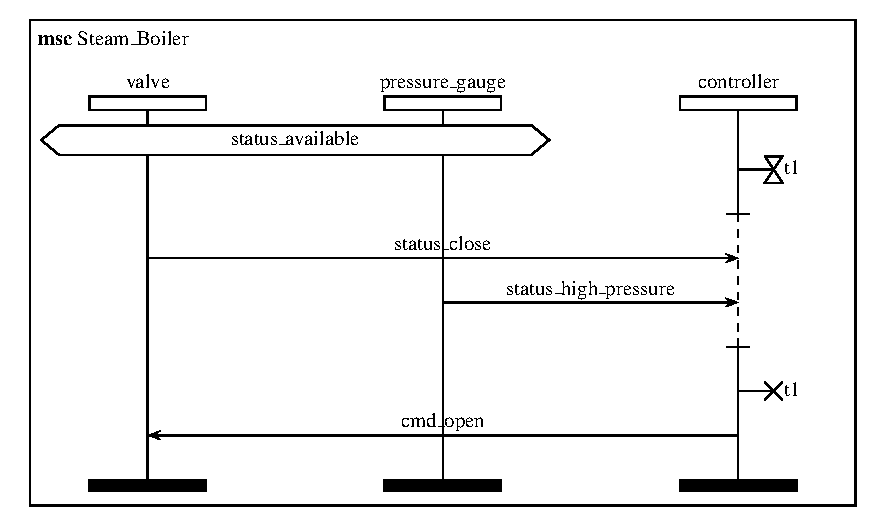
\includegraphics[width=10cm]{fig2}
%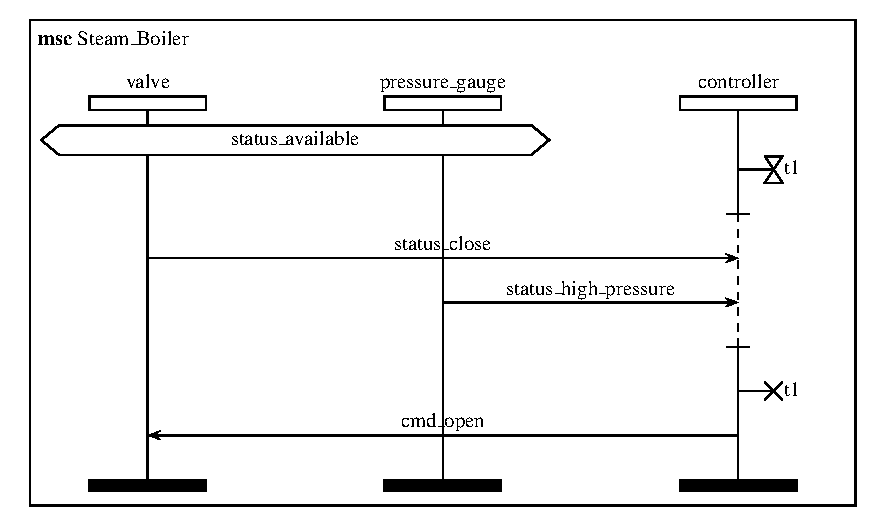
\includegraphics{fig2}
\caption{Basic MSC}
\label{fig2}
\end{figure*}

Figure~\ref{fig2} shows an MSC that depicts a simple interaction 
among 3 instances named $valve$, $controller$ and 
$pressure\_gauge$. Each vertical line for an instance 
denotes the events that happen within the instance; the 
topmost event is the earliest event (within the 
instance) and so on downwards in time. This temporal 
ordering of events for an instance is called its 
{\em local order}. The visual distance between the 
events within a local order is immaterial. In Figure~\ref{fig2}, 
the $valve$ and $pressure\_gauge$ processes 
send their respective status to the $controller$ 
using messages named $status\_close$ and 
$status\_high\_pressure$ respectively. The $controller$ 
then issues an open command to the $valve$ using the 
message named $cmd\_open$. Note that the MSC depicts 
only one scenario; many other scenarios are possible 
e.g., one where the valve is open, pressure is 
low and the controller issues command to close the 
valve. The MSC is enclosed in a rectangular frame 
and has a name ($Steam\_Boiler$ in this example).

The MSC notation allows one to avoid any particular 
ordering of a subset of events for a process, by 
using a construct called co-region. A {\em co-region} 
is indicated by a dotted line segment along the 
vertical line for the process and the events within 
this dotted line are unordered. Figure~\ref{fig2} shows 
a co-region for $controller$ in which the $controller$ 
does not impose any order on the receipt of the 
$status\_close$ message from $valve$ and 
$status\_high\_pressure$ message from $pressure\_gauge$ 
(these messages may be received in any order).

Many scenarios relate message flows with timing 
constraints. It is possible to easily specify such 
scenarios in the MSC notation using three special 
events: timer set, timer reset and timeout. The 
{\em timer set} event is denoted by an hourglass 
symbol connected to the timeline of a single process. 
The {\em timer reset} event is denoted by a cross 
connected to the timeline of a process. The 
{\em timeout} event is denoted by connecting the 
hourglass symbol of the timer to the process timeline 
by a bent line. Each timer has a unique name. 
Naturally, for each timer, the timer reset and timeout 
events must be preceded by the timer set event. In 
Figure~\ref{fig2}, the controller starts a timer $t1$ before 
waiting for the messages from $valve$ and 
$pressure\_gauge$ instances. In this particular 
scenario, the $controller$ receives both the 
messages before the timeout and then resets the 
timer $t1$.

A {\em condition} is an informal descriptive 
mechanism in the MSC notation used to display a state 
or situation that must be reached by either a single 
instance or a group of instances. A condition is 
written as a text label within a hexagonal box, which 
is placed either on a single instance or across a 
group of instances. If a condition $C$ is placed on 
a single instance $P$ then the execution of $P$ does 
not proceed to the next event (below the condition 
on the local order) until the condition is reached. 
That is, the condition $C$ is a pre-requisite for 
the next event in the instance. If the condition 
$C$ is placed across a group of instances 
$P_1,\ldots,P_k$, then all the $k$ instances must 
achieve local states in which the condition $C$ 
is satisfied; only after that state is reached, 
can any of the $k$ instances proceed further in 
their respective local orders. In such a case, 
the condition $C$ can be thought of a 
synchronisation mechanism useful to ensure that 
the instances $P_1,\ldots,P_k$ reach the same state 
before proceeding further. In Figure~\ref{fig2}, instances 
$valve$ and $pressure\_gauge$ share a condition 
called $status\_available$; only when 
both these instances reach a state that satisfies 
this condition, can they proceed further with 
their local orders.

What exactly is the scenario specified by the 
basic MSC in Figure~\ref{fig2}? It may appear that the 
MSC represents only one sequence of events; in fact 
it represents several actual event sequences each 
of which {\em captures} the intended behaviour. 
To understand this clearly, we formally define 
the linear time semantics of a basic MSC.

\subsection{Linear Time Semantics of Basic MSCs}

The MSC notation discussed so far is called a basic MSC 
to distinguish it from the HMSC defined later. 
We now formally define the linear time semantics 
of a basic MSC in terms of the associated partial 
order and the set of runs~\cite{Alur96,DammHarel99,BVP02}. With 
each instance $i$ in a given basic MSC $m$, we 
associate an ordered sequence $0 .. lmax(m,i)$ 
of finite number of discrete locations, which 
are numbered from the top of the instance to 
the bottom. Each location on an instance $i$ in 
basic MSC $m$, denoted $<i,l>_m$, is associated 
with an event, which may be sending or receiving 
of a message, a condition, or timer events set, 
reset, timeout. We drop the subscript $m$ when 
the basic MSC is clear from the context. The 
semantics of a basic MSC $m$ is defined in terms 
of the partial order $\leq_m$ induced by $m$ on 
the set of its locations $<i,l>$. The partial 
order is obtained from the following precedence 
relation $R_m$:
\begin{itemize}
\item visual order along an instance line: 
$<i,l> R_m <i,l+1>$ unless the two consecutive 
locations are in a co-region
\item send of a message precedes its receipt: 
if $<i,l>$ is a send event and $<i',l'>$ is the 
corresponding receive event for the message, 
then $<i,l> R_m <i',l'>$
\item shared condition induces synchronisation 
barrier: if locations $<i,l>$ and $<i',l'>$ 
refer to the same condition $c$, then 
$<i,l> R_m <i',l'+1>$
\item events within a co-region have no order 
among them: suppose $<i,l>,<i,l+1>,\ldots,<i,l+k>$ 
are events in a co-region. If $l > 0$ (i.e., 
there is at least one event before the co-region) 
then $<i,l-1> R_m <i,l>$, $<i,l-1> R_m <i,l+1>$,
\ldots,$<i,l-1> R_m <i,l+k>$. Also, if $k < lmax(i,m)$ 
(i.e., there is at least one event after the co-region) 
then $<i,l> R_m <i,l+k+1>$,$<i,l+1> R_m <i,l+k+1>$,
\ldots,$<i,l+k> R_m <i,l+k+1>$.
\end{itemize}

We assume that the basic MSC $m$ is well-formed 
so that the relation $R_m$ is acyclic. We call 
$R_m$ the {\em precedence relation} of the basic 
MSC $m$. The partial order $\leq_m$ is the 
reflexive transitive closure of $R_m$.

\begin{definition}
\label{bmscsem}
The semantics of a basic MSC $m$ is the set of all 
runs (i.e., linearizations) of the partial order 
$\leq_m$.
\end{definition}

This implies that we have interleaving semantics 
for concurrency: any two events that are 
incomparable in the partial order can happen in 
any order. Note also that each run of a basic 
MSC is a finite sequence of events and each 
basic MSC has only a finite number of such 
finite runs. The precedence graph in Figure~\ref{fig3} 
depicts the precedence relation $R_m$ among the 
locations (events) in the basic MSC of Figure~\ref{fig2}. 
The vertices of this precedence graph stand for 
events; there is a directed edge from event $u$ 
to event $v$ if $u$ directly precedes $v$ i.e., 
$u R_m v$. An event $v$ cannot {\em occur} until 
all preceding events have occurred. If the MSC 
is well-formed then the corresponding precedence 
graph is a directed acyclic graph (DAG).

\begin{figure*}[t]
\centering
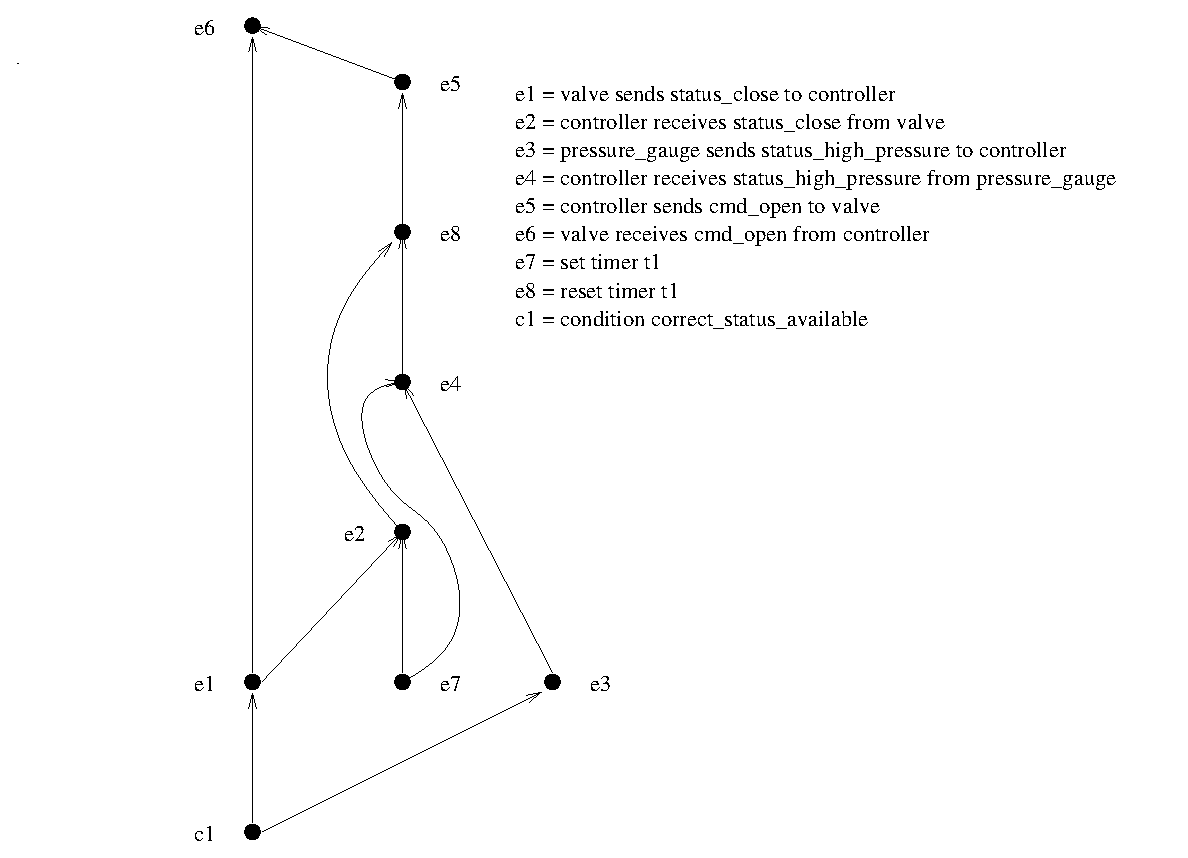
\includegraphics[height=10cm]{fig3}
%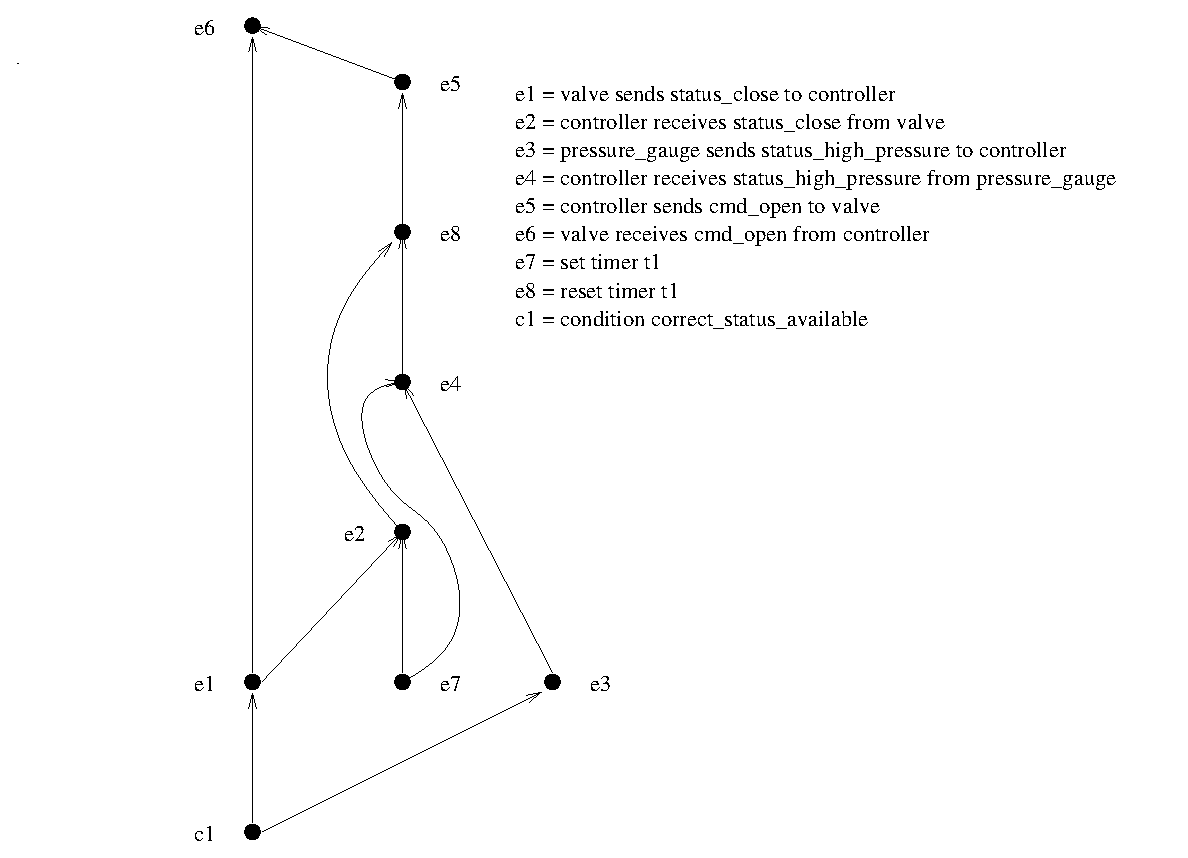
\includegraphics{fig3}
\caption{Precedence graph for the basic MSC in Figure~\ref{fig2}}
\label{fig3}
\end{figure*}

\bibliographystyle{entcs}
%\bibliography{pbhaduri}

\begin{thebibliography}{10}
\expandafter\ifx\csname url\endcsname\relax
  \def\url#1{\texttt{#1}}\fi
\expandafter\ifx\csname urlprefix\endcsname\relax\def\urlprefix{URL }\fi
\newcommand{\enquote}[1]{``#1''}

\bibitem{AEY01b}
Alur, R., K.~Etessami and M.~Yannakakis, \emph{Realizability and verification
  of {MSC} graphs}, in: \emph{Proc. 28th Int. Col. on Automata, Languages and
  Programming}, 2001, pp. 797--808.

\bibitem{Alur96}
Alur, R., G.~Holzmann and D.~Peled, \emph{{An Analyzer for Message Sequence
  Charts}}, Software Concepts and Tools \textbf{17} (1996), pp.~70--77.

\bibitem{AlurYannakakis99}
Alur, R. and M.~Yannakakis, \emph{{M}odel {C}hecking of {M}essage {S}equence
  {C}harts}, in: \emph{Proceedings of the Tenth International Conference on
  Concurrency Theory, CONCUR'99}, Lecture Notes in Computer Science (1999).

\bibitem{1997:tacas:ben-abdallah}
Ben-Abdallah, H. and S.~Leue, \emph{Syntactic detection of process divergence
  and non-local choice in message sequence charts}, in: E.~Brinksma, editor,
  \emph{Tools and Algorithms for the Construction and Analysis of Systems},
  Lecture Notes in Computer Science  \textbf{1217} (1997), pp. 259--274.

\bibitem{BVP02}
Bhaduri, P., R.~Venkatesh and G.~Palshikar, \emph{Formal techniques for
  analysing scenarios using message sequence charts}, in: \emph{ETAPS Workshop
  on Validation and Implementation of Scenario-based Specifications, VISS 2002,
  Grenoble}, 2002, appeared in Electronic Notes in Theoretical Computer
  Science, Volume 65, Issue 7, Elsevier,
  \url{http://www.elsevier.com/gej-ng/31/29/23/117/50/26/65.7.002.pdf}.

\bibitem{DammHarel99}
Damm, W. and D.~Harel, \emph{{LSCs}: Breathing {L}ife into {M}essage {S}equence
  {C}harts}, in: \emph{FMOODS'99: Proc. Third IFIP Intl. Conf. on Formal
  Methods for Open Object-Based Distributed Systems}, 1999.

\bibitem{patterns-spec}
Dwyer, M., G.~Avrunin and J.~Corbett, \emph{Property specification patterns for
  finite-state verification}, in: \emph{Proceedings of the Second Workshop on
  Formal Methods in Software Practice}, 1998, pp. 7--15.

\bibitem{Feijs00}
Feijs, L.~M., \emph{Natural language and message sequence chart representation
  of use cases}, Information and Software Technology \textbf{42} (2000),
  pp.~633--647.

\bibitem{gehrke98algebraic}
Gehrke, T., M.~Huhn, A.~Rensink and H.~Wehrheim, \emph{An algebraic semantics
  for message sequence chart documents}, in: \emph{{FORTE}}, 1998, pp. 3--18.

\bibitem{GenestEtAl02}
Genest, B., A.~Muscholl, H.~Seidl and M.~Zeitoun, \emph{Infinite-state
  high-level {MSC}s: Model-checking and realizability}, in: \emph{ICALP: Annual
  International Colloquium on Automata, Languages and Programming}, 2002, pp.
  657--668.

\bibitem{Graubmann:2000:UML}
Graubmann, P. and E.~Rudolph, \emph{Hypermscs and sequence diagrams for use
  case modelling and testing}, in: A.~Evans, S.~Kent and B.~Selic, editors,
  \emph{UML 2000 - The Unified Modeling Language. Advancing the Standard. Third
  International Conference, York, UK, October 2000, Proceedings},  LNCS
  \textbf{1939} (2000), pp. 32--46.

\bibitem{Haugen:SDL:2001}
Haugen, {\O}., \emph{From {MSC-2000} to {UML 2.0} - {The} future of sequence
  diagrams}, in: \emph{SDL 2001: Meeting UML. 10th International SDL Forum
  Copenhagen, Denmark, June 27-29, 2001, Proceedings},  LNCS  \textbf{2078}
  (2001), pp. 38--51.

\bibitem{Haugen:2001:MID}
Haugen, {\O}., \emph{{MSC}-2000 interaction diagrams for the new millennium},
  Computer Networks (Amsterdam, Netherlands: 1999) \textbf{35} (2001),
  pp.~721--732.

\bibitem{MSC96}
ITU-T, \emph{{ITU-T Recommendation Z.120: Message Sequence Chart (MSC)}}
  (1996).

\bibitem{model-checking-managers}
Janssen, W., R.~Mateescu, S.~Mauw, P.~Fennema and P.~van~der Stappen,
  \emph{Model checking for managers}, in: \emph{Proceedings of the 6th
  International SPIN Workshop on Practical Aspects of Model Checking (Toulouse,
  France)}, 1999.

\bibitem{Jonsson:2001:ESM}
Jonsson, B. and G.~Padilla, \emph{An execution semantics for {MSC-2000}},
  Lecture Notes in Computer Science \textbf{2078} (2001), pp.~365--378.

\bibitem{LevPel97}
Levin, V. and D.~Peled, \emph{Verification of message sequence charts via
  template matching}, in: \emph{TAPSOFT (FASE)'97, Theory and Practice of
  Software Development},  LNCS  \textbf{1214} (1997), pp. 652--666.

\bibitem{Mauw96}
Mauw, S., \emph{{The Formalization of Message Sequence Charts}}, Computer
  Networks and ISDN Systems \textbf{28} (1996).

\bibitem{Mauw:1999:OSM}
Mauw, S. and M.~A. Reniers, \emph{Operational {Semantics} for {MSC'96}},
  Computer Networks (Amsterdam, Netherlands: 1999) \textbf{31} (1999),
  pp.~1785--1799.

\bibitem{Miga:2001:DMS}
Miga, A., D.~Amyot, F.~Bordeleau, D.~Cameron and M.~Woodside, \emph{Deriving
  message sequence charts from use case maps scenario specifications}, Lecture
  Notes in Computer Science \textbf{2078} (2001), pp.~268--287.

\bibitem{MuschollPeled00}
Muscholl, A. and D.~Peled, \emph{Analyzing message sequence charts}, in:
  \emph{Proc. of SAM'00, Grenoble}, 2000.

\bibitem{MSP98}
Muscholl, A., Z.~Su and D.~Peled, \emph{Deciding properties for message
  sequence charts}, in: \emph{FoSSaCS, Foundations of Software Science and
  Computation Structures}, Lisbon, Portugal, 1998.

\bibitem{Girish03}
Palshikar, G.~K., A.~Pavaskar, M.~Jadhav, D.~Patil and M.~Bakshi, \emph{An
  {RF}-based embedded system for protecting unmanned railway crossings}, in:
  \emph{Conference on Information Technology (CIT 2003), Bhubaneshwar}, 2003.

\bibitem{Peled00}
Peled, D., \emph{Specification and verification of message sequence charts},
  in: \emph{Proc. IFIP FORTE/PSTV}, 2000, pp. 139--154.

\bibitem{Rudolph96a}
Rudolph, E., J.~Grabowski and P.~Graubmann, \emph{{Tutorial on Message Sequence
  Charts}}, Computer Networks and ISDN Systems \textbf{28} (1996),
  pp.~1629--1641.

\bibitem{Silva98}
Silva, P. S.~M., \emph{Extended {Message Sequence Charts} with time-interval
  semantics}, in: \emph{5th Workshop on Temporal Representation and Reasoning,
  TIME '98}, 1998, pp. 37--44.

\end{thebibliography}

\end{document}

